\subsection{Teilmengenkonsstruktion (Arbeitslistenalgorithmus)}
\begin{enumerate}
    \item Zeichne eine Tabelle(DEA, Zustände, NEA)
    \item Starte mit dem Startsymbol und führe einen neuen Zustand ein.
    \item Folge den Produktionen des Startzutands und erzeuge für die erreichbare Zustände durch ein Terminalsymbol im DEA, einen neuen Zustand.
    \item Wiederhole die Suche nach erreichbaren Zuständen für alle anderen Zustände des erzeugten DEAs, solange bis sich nichts mehr ändert
\end{enumerate}
\begin{center}
    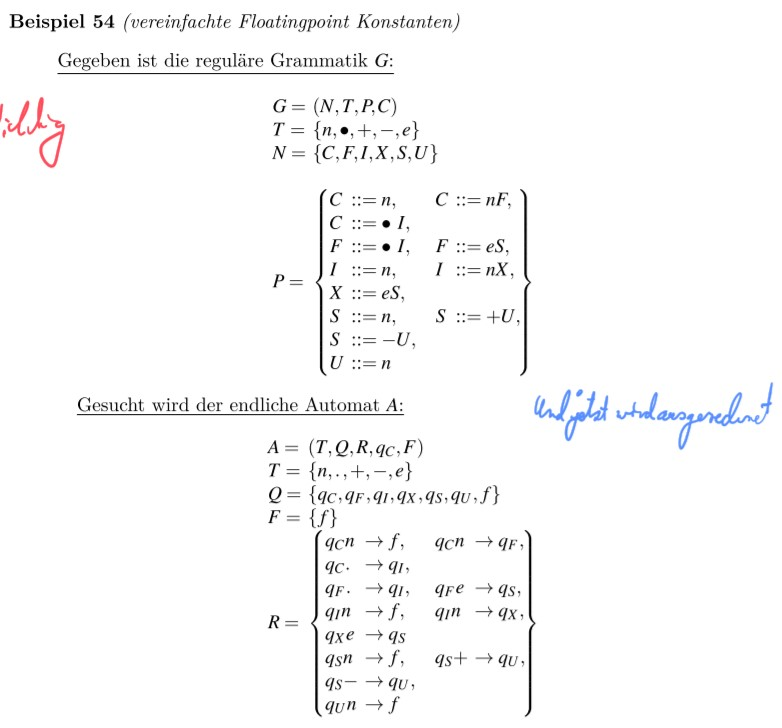
\includegraphics[height=7.5cm]{image/Tabelle_Teilmengen.jpg}
  \end{center}